\section{Discussion}
\label{sec:discussion}
\subsection{Implications of anomalous Tor keys}
\paragraph{Implications for the network}
As touched on earlier in Section~\ref{sec:tor-network}, the main use of the
identity key in Tor is to sign the relay's descriptor, which includes various
information about the relay, \eg, its IP address and contact information.
Relays publish their public identity keys in their descriptor.  The network
consensus acts as the public key infrastructure of Tor.  Signed by the directory
authorities whose public keys are hard-coded in Tor's source code, the network
consensus points to the descriptors of each Tor relay that is currently online.
If an attacker were to break the identity key of a relay (as we demonstrated),
she could start signing descriptors in the relay's name and publishing them. The
adversary could publish whatever information she wanted in the descriptor, \eg
her own IP address, keys, \etc, in order to fool Tor clients.  In other words,
weak keys allow adversaries to obtain the affected relay's reputation which
matters because Tor clients make routing decisions based on this reputation.

The Tor protocol's use of forward secrecy mitigates the potential harm of weak
keys.  Recall that a relay's long-lived identity keys are only used to sign
data, so forward secrecy does not apply here.  Onion keys however are used for
decryption and encryption, and are rotated by default each 28
days~\cite[\S~3.4.1]{dir-spec}.  An attacker who managed to compromise a weak
onion key is still faced with the underlying TLS layer, shown in
Figure~\ref{fig:protostack}, that provides defense in depth.  The Tor
specification requires the keys for the TLS layer to be rotated at least once a
day~\cite[\S~1.1]{torspec}, making it difficult to get any use out of
compromised onion keys.

\begin{figure}
\centering
% Change arrow head globally.
\tikzset{>=latex}
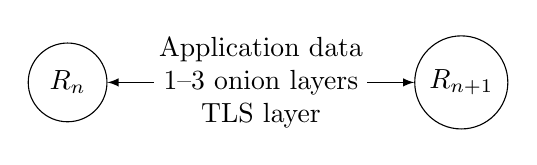
\begin{tikzpicture}

\node[circle,draw,minimum size=1cm] (R1) at (0, 0) {$R_n$};
\node[circle,draw,minimum size=1cm] (R2) at (5, 0) {$R_{n+1}$};

\draw[<->] (R1.east) -- node [midway, fill=white] (line) {\phantom{1--3 onion layers}} (R2.west);

\node[align=center] at (line) {Application data\\1--3 onion layers\\TLS layer};

\end{tikzpicture}
\caption{The protocol stack between two Tor relays $R_n$ and $R_n+1$.  The
lowest layer is a TLS connection that contains one (between the middle and exit
relay) to three (between the client and guard relay) onion layers.  The onion
layers protect the application data that the client is sending.}
\label{fig:protostack}
\end{figure}

\paragraph{Implications for Tor users}
To understand how Tor users are affected by weak keys we need to distinguish
between \emph{targeting} and \emph{hoovering} adversaries.\footnote{We here use
Jaggard and Syverson's nomenclature of an adversary that either targets
specific Tor users (targeting) or hoovers up all available data to
deanonymize as many users as possible (hoovering)~\cite{Jaggard2017a}.}
The goal of targeting adversaries is to focus an attack on a small number of
users among the large set of all Tor users.  Generally speaking, weak keys can
be problematic in a targeted setting if they allow an attacker to gain access to
a Tor relay she would otherwise be unable to control.  This can be the case if
the attacker learned the targeted user's guard relay and can the guard happens
to have weak keys.  However, judging by our experimental results, the
probability of an attacker knowing a targeted user's guard relay \emph{and} this
guard relay having vulnerable keys is very low.

Hoovering adversaries are opportunistic by definition and seek to deanonymize as
many Tor users as possible.  Recall that Tor clients use a long-lived guard
relay as their first hop and two randomly chosen relays for the next two
hops.\footnote{We refer to these relays as randomly chosen for simplicity but
the path selection algorithm is more complicated.}  A single compromised relay
is not necessarily harmful to users but weak keys can be a problem if a user
happens to have a guard relay with weak keys \emph{and} selects an exit relay
that also has weak keys, allowing the hoovering adversary to deanonymize the
circuit.  Again, considering the low prevalence of weak keys and the ease with
which The Tor Project could identify and block relays with weak keys, hoovering
adversaries pose no significant threat.

\subsection{Preventing non-standard exponents}
Recall that the Tor reference implementation hard-codes its public RSA exponent
to 65,537~\cite[\S~0.3]{torspec}.  The Tor Project could prevent non-standard
exponents by having the directory authorities reject relays whose descriptors
have an RSA exponent other than 65,537, thus slowing down the search for
fingerprint prefixes.  Adversaries would then have to iterate over the primes
$p$ or $q$ instead of the exponent, rendering the search computationally
more expensive because of the cost of primality tests.  Given that we discovered
only 122 unusual exponents in over ten years of data, we believe that rejecting
non-standard exponents is a viable defense in depth.

\subsection{Analyzing onion service public keys}
Future work should shed light on the public keys of onion services.  Onion
services have an incentive to modify their fingerprints to make them both
recognizable and easier to remember.  Facebook, for example, was lucky to
obtain the easy-to-remember onion domain
\url{facebookcorewwwi.onion}~\cite{facebook}.  The tool Scallion assists onion
service operators in creating such vanity domains~\cite{scallion}.  The
implications of vanity domains on usability and security are still poorly
understood~\cite{vanity-domains}.  Unlike the public keys of relays, onion
service keys are not archived, so a study would have to begin with actively
fetching onion service keys.

\subsection{\textit{In vivo} Tor research}
Caution must be taken when conducting research using the live Tor network.
Section~\ref{sec:shared-primes} showed how a small mistake in key generation led
to many vulnerable Tor relays.  To keep its users safe, The Tor Project has
recently launched a research safety board whose aim is to assist researchers in
safely conducting Tor measurement studies~\cite{safety-board}.  This may entail
running experiments in private Tor networks that are controlled by the
researchers, or using network simulators such as Shadow~\cite{Jansen2012a}.

As for our own work, we were in close contact with Tor developers throughout our
research effort and shared preliminary results as we progressed.  Once we wrote
up our findings in a technical report we brought it to the broader Tor
community's attention by sending an email to the tor-dev mailing
list~\cite{Roberts2017a}.  On top of that we adopted open science practices and
wrote both our code and paper in the open, allowing interested parties to
immediately learn about any progress.

\subsection{The effect of next-generation onion services}
As of August 2017, The Tor Project is finalizing the design of next-generation
onion services~\cite{prop224}.  In addition to stronger cryptographic
primitives, the design fixes the issue of predicting an onion service's location
in the hash ring by incorporating a random element.  This element is produced by
having the directory authorities agree on a random number once a
day~\cite{prop250}.  The random number is embedded in the consensus document and
used by clients to fetch an onion service's descriptor.  Attackers will no
longer be able to attack onion services by positioning HSDirs in the hash ring;
while they have several hours to compute a key pair that positions their HSDirs
next to the onion service's descriptor, it takes at least 96 hours to get the
HSDir flag from the directory authorities~\cite[\S~3.4.2]{dir-spec}.  We expect
this design change to disincentivize attackers from manipulating their keys to
attack onion services.
